\documentclass{standalone}
\usepackage{tikz}
\usetikzlibrary{patterns, positioning}
\usepackage[sfdefault]{ClearSans} %% option 'sfdefault' activates Clear Sans as the default text font
\usepackage[T1]{fontenc}

\begin{document}
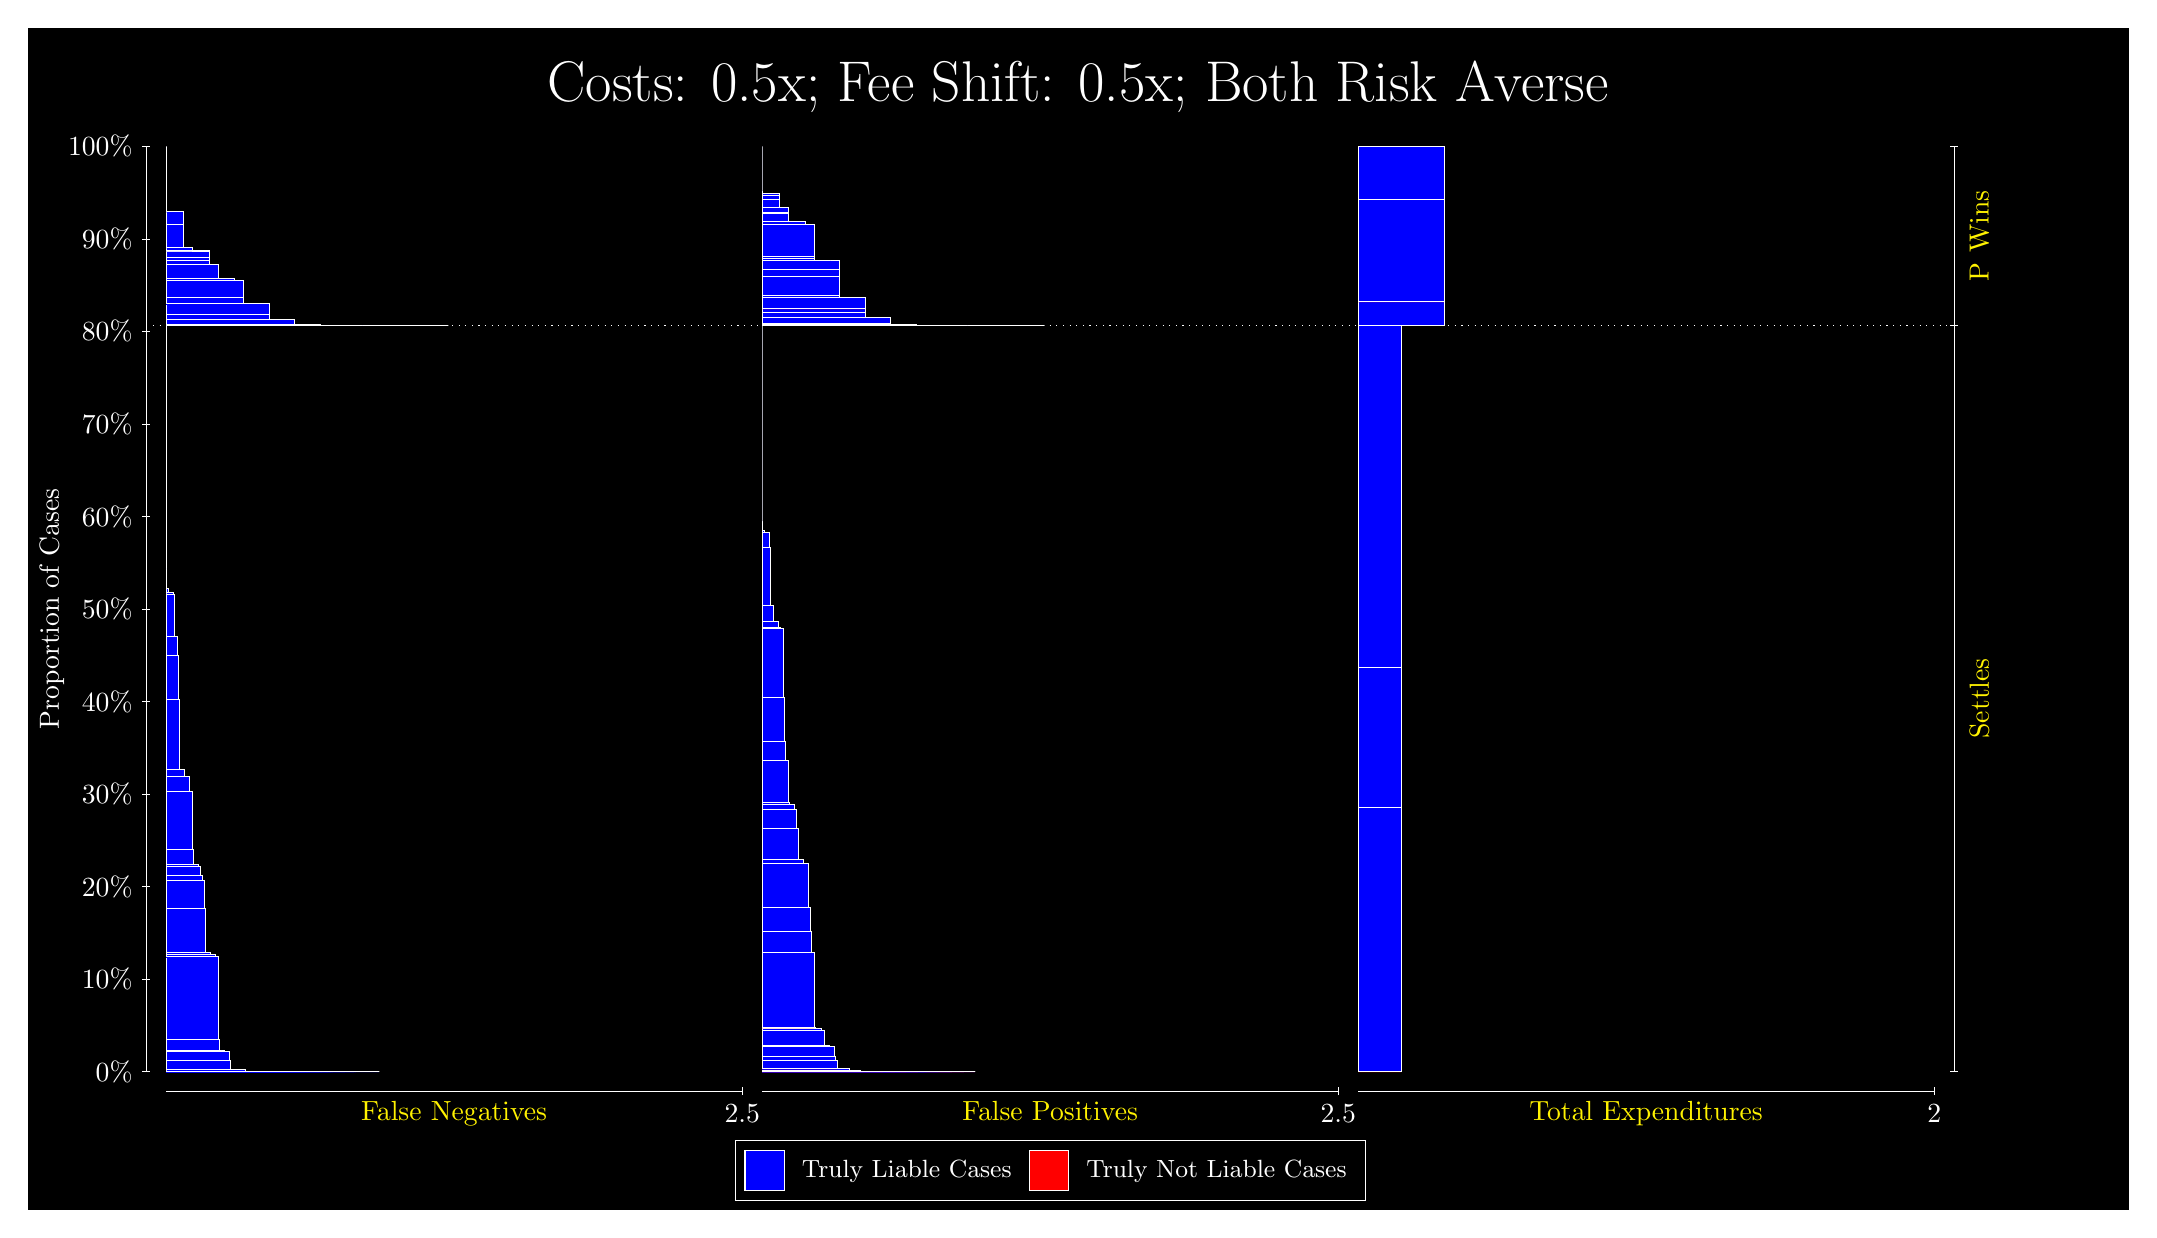
\begin{tikzpicture}
\draw[fill=black] (0,0) rectangle (26.667,15);
\draw[text=white] (0,13.5) rectangle (26.667,15) node[midway] {\huge Costs: 0.5x; Fee Shift: 0.5x; Both Risk Averse};
\draw[white, very thin] (1.5,1.75) -- (1.5,13.5);
\node[rotate=90, text=white, anchor=center] at (0.3, 7.625) {Proportion of Cases};
\draw[white, very thin] (1.45,1.75) -- (1.55,1.75);
\node[text=white, anchor=east] at (1.45, 1.75) {0\%};
\draw[white, very thin] (1.45,2.925) -- (1.55,2.925);
\node[text=white, anchor=east] at (1.45, 2.925) {10\%};
\draw[white, very thin] (1.45,4.1) -- (1.55,4.1);
\node[text=white, anchor=east] at (1.45, 4.1) {20\%};
\draw[white, very thin] (1.45,5.275) -- (1.55,5.275);
\node[text=white, anchor=east] at (1.45, 5.275) {30\%};
\draw[white, very thin] (1.45,6.45) -- (1.55,6.45);
\node[text=white, anchor=east] at (1.45, 6.45) {40\%};
\draw[white, very thin] (1.45,7.625) -- (1.55,7.625);
\node[text=white, anchor=east] at (1.45, 7.625) {50\%};
\draw[white, very thin] (1.45,8.8) -- (1.55,8.8);
\node[text=white, anchor=east] at (1.45, 8.8) {60\%};
\draw[white, very thin] (1.45,9.975) -- (1.55,9.975);
\node[text=white, anchor=east] at (1.45, 9.975) {70\%};
\draw[white, very thin] (1.45,11.15) -- (1.55,11.15);
\node[text=white, anchor=east] at (1.45, 11.15) {80\%};
\draw[white, very thin] (1.45,12.325) -- (1.55,12.325);
\node[text=white, anchor=east] at (1.45, 12.325) {90\%};
\draw[white, very thin] (1.45,13.5) -- (1.55,13.5);
\node[text=white, anchor=east] at (1.45, 13.5) {100\%};

\draw[white, very thin] (24.457,1.75) -- (24.457,13.5);
\draw[white, very thin] (24.407,1.75) -- (24.507,1.75);
\node[anchor=west] at (24.407, 1.75) {};
\draw[white, very thin] (24.407,11.228) -- (24.507,11.228);
\node[anchor=west] at (24.407, 11.228) {};
\draw[white, very thin] (24.407,13.5) -- (24.507,13.5);
\node[anchor=west] at (24.407, 13.5) {};

\draw[white, very thin, fill=blue] (1.75,1.75) rectangle (4.458,1.75);
\draw[white, very thin, fill=blue] (1.75,1.75) rectangle (4.1652,1.75);
\draw[white, very thin, fill=blue] (1.75,1.75) rectangle (4.1327,1.75);
\draw[white, very thin, fill=blue] (1.75,1.75) rectangle (4.0188,1.75);
\draw[white, very thin, fill=blue] (1.75,1.75) rectangle (3.8725,1.75);
\draw[white, very thin, fill=blue] (1.75,1.75) rectangle (3.8399,1.75);
\draw[white, very thin, fill=blue] (1.75,1.75) rectangle (3.8074,1.75);
\draw[white, very thin, fill=blue] (1.75,1.75) rectangle (3.7261,1.75);
\draw[white, very thin, fill=blue] (1.75,1.75) rectangle (3.6936,1.75);
\draw[white, very thin, fill=blue] (1.75,1.75) rectangle (3.5797,1.75);
\draw[white, very thin, fill=blue] (1.75,1.75) rectangle (3.5472,1.75);
\draw[white, very thin, fill=blue] (1.75,1.75) rectangle (3.5147,1.75);
\draw[white, very thin, fill=blue] (1.75,1.75) rectangle (3.4821,1.75);
\draw[white, very thin, fill=blue] (1.75,1.75) rectangle (3.4333,1.75);
\draw[white, very thin, fill=blue] (1.75,1.75) rectangle (3.4008,1.75);
\draw[white, very thin, fill=blue] (1.75,1.75) rectangle (3.3683,1.75);
\draw[white, very thin, fill=blue] (1.75,1.75) rectangle (3.287,1.75);
\draw[white, very thin, fill=blue] (1.75,1.75) rectangle (3.2544,1.75);
\draw[white, very thin, fill=blue] (1.75,1.75) rectangle (3.2219,1.75);
\draw[white, very thin, fill=blue] (1.75,1.75) rectangle (3.1894,1.75);
\draw[white, very thin, fill=blue] (1.75,1.75) rectangle (3.1568,1.75);
\draw[white, very thin, fill=blue] (1.75,1.75) rectangle (3.1406,1.7501);
\draw[white, very thin, fill=blue] (1.75,1.7501) rectangle (3.1081,1.7501);
\draw[white, very thin, fill=blue] (1.75,1.7501) rectangle (3.0755,1.7505);
\draw[white, very thin, fill=blue] (1.75,1.7505) rectangle (3.043,1.7505);
\draw[white, very thin, fill=blue] (1.75,1.7505) rectangle (2.9617,1.7505);
\draw[white, very thin, fill=blue] (1.75,1.7505) rectangle (2.9292,1.7505);
\draw[white, very thin, fill=blue] (1.75,1.7505) rectangle (2.8966,1.7558);
\draw[white, very thin, fill=blue] (1.75,1.7558) rectangle (2.8641,1.7559);
\draw[white, very thin, fill=blue] (1.75,1.7559) rectangle (2.8316,1.7559);
\draw[white, very thin, fill=blue] (1.75,1.7559) rectangle (2.8153,1.7562);
\draw[white, very thin, fill=blue] (1.75,1.7562) rectangle (2.7828,1.7562);
\draw[white, very thin, fill=blue] (1.75,1.7562) rectangle (2.7502,1.7752);
\draw[white, very thin, fill=blue] (1.75,1.7752) rectangle (2.7177,1.7753);
\draw[white, very thin, fill=blue] (1.75,1.7753) rectangle (2.7015,1.7762);
\draw[white, very thin, fill=blue] (1.75,1.7762) rectangle (2.6364,1.778);
\draw[white, very thin, fill=blue] (1.75,1.778) rectangle (2.6039,1.778);
\draw[white, very thin, fill=blue] (1.75,1.778) rectangle (2.5713,1.8897);
\draw[white, very thin, fill=blue] (1.75,1.8897) rectangle (2.5551,2.0022);
\draw[white, very thin, fill=blue] (1.75,2.0022) rectangle (2.5388,2.0072);
\draw[white, very thin, fill=blue] (1.75,2.0072) rectangle (2.5063,2.0124);
\draw[white, very thin, fill=blue] (1.75,2.0124) rectangle (2.49,2.0175);
\draw[white, very thin, fill=blue] (1.75,2.0175) rectangle (2.4575,2.0175);
\draw[white, very thin, fill=blue] (1.75,2.0175) rectangle (2.425,2.1562);
\draw[white, very thin, fill=blue] (1.75,2.1562) rectangle (2.4087,3.2082);
\draw[white, very thin, fill=blue] (1.75,3.2082) rectangle (2.3924,3.2099);
\draw[white, very thin, fill=blue] (1.75,3.2099) rectangle (2.3762,3.2351);
\draw[white, very thin, fill=blue] (1.75,3.2351) rectangle (2.3111,3.2652);
\draw[white, very thin, fill=blue] (1.75,3.2652) rectangle (2.2786,3.2653);
\draw[white, very thin, fill=blue] (1.75,3.2653) rectangle (2.2461,3.817);
\draw[white, very thin, fill=blue] (1.75,3.817) rectangle (2.2298,4.1774);
\draw[white, very thin, fill=blue] (1.75,4.1774) rectangle (2.2135,4.2452);
\draw[white, very thin, fill=blue] (1.75,4.2452) rectangle (2.181,4.354);
\draw[white, very thin, fill=blue] (1.75,4.354) rectangle (2.1647,4.3782);
\draw[white, very thin, fill=blue] (1.75,4.3782) rectangle (2.1322,4.3782);
\draw[white, very thin, fill=blue] (1.75,4.3782) rectangle (2.0997,4.5728);
\draw[white, very thin, fill=blue] (1.75,4.5728) rectangle (2.0834,5.3031);
\draw[white, very thin, fill=blue] (1.75,5.3031) rectangle (2.0672,5.3078);
\draw[white, very thin, fill=blue] (1.75,5.3078) rectangle (2.0509,5.5049);
\draw[white, very thin, fill=blue] (1.75,5.5049) rectangle (1.9858,5.5925);
\draw[white, very thin, fill=blue] (1.75,5.5925) rectangle (1.9533,5.5929);
\draw[white, very thin, fill=blue] (1.75,5.5929) rectangle (1.9208,6.4753);
\draw[white, very thin, fill=blue] (1.75,6.4753) rectangle (1.9045,7.034);
\draw[white, very thin, fill=blue] (1.75,7.034) rectangle (1.8882,7.2804);
\draw[white, very thin, fill=blue] (1.75,7.2804) rectangle (1.8557,7.8069);
\draw[white, very thin, fill=blue] (1.75,7.8069) rectangle (1.8395,7.8311);
\draw[white, very thin, fill=blue] (1.75,7.8311) rectangle (1.8069,7.8312);
\draw[white, very thin, fill=blue] (1.75,7.8312) rectangle (1.7744,7.8929);
\draw[white, very thin, fill=blue] (1.75,7.8929) rectangle (1.7581,8.1393);
\draw[white, very thin, fill=red] (1.75,8.1393) rectangle (1.75,8.1393);
\draw[white, very thin, fill=blue] (1.75,8.1393) rectangle (1.75,11.228);
\draw[white, very thin, fill=blue] (1.75,11.228) rectangle (5.3362,11.228);
\draw[white, very thin, fill=blue] (1.75,11.228) rectangle (5.011,11.228);
\draw[white, very thin, fill=blue] (1.75,11.228) rectangle (4.6857,11.228);
\draw[white, very thin, fill=blue] (1.75,11.228) rectangle (4.3604,11.229);
\draw[white, very thin, fill=blue] (1.75,11.229) rectangle (4.2465,11.229);
\draw[white, very thin, fill=blue] (1.75,11.229) rectangle (4.0351,11.229);
\draw[white, very thin, fill=blue] (1.75,11.229) rectangle (4.0351,11.23);
\draw[white, very thin, fill=blue] (1.75,11.23) rectangle (3.9213,11.23);
\draw[white, very thin, fill=blue] (1.75,11.23) rectangle (3.7098,11.236);
\draw[white, very thin, fill=blue] (1.75,11.236) rectangle (3.7098,11.243);
\draw[white, very thin, fill=blue] (1.75,11.243) rectangle (3.596,11.243);
\draw[white, very thin, fill=blue] (1.75,11.243) rectangle (3.3845,11.304);
\draw[white, very thin, fill=blue] (1.75,11.304) rectangle (3.3845,11.306);
\draw[white, very thin, fill=blue] (1.75,11.306) rectangle (3.2707,11.306);
\draw[white, very thin, fill=blue] (1.75,11.306) rectangle (3.2707,11.306);
\draw[white, very thin, fill=blue] (1.75,11.306) rectangle (3.0593,11.369);
\draw[white, very thin, fill=blue] (1.75,11.369) rectangle (3.0593,11.502);
\draw[white, very thin, fill=blue] (1.75,11.502) rectangle (2.9454,11.502);
\draw[white, very thin, fill=blue] (1.75,11.502) rectangle (2.9454,11.502);
\draw[white, very thin, fill=blue] (1.75,11.502) rectangle (2.9454,11.503);
\draw[white, very thin, fill=blue] (1.75,11.503) rectangle (2.734,11.588);
\draw[white, very thin, fill=blue] (1.75,11.588) rectangle (2.734,11.796);
\draw[white, very thin, fill=blue] (1.75,11.796) rectangle (2.734,11.802);
\draw[white, very thin, fill=blue] (1.75,11.802) rectangle (2.6201,11.802);
\draw[white, very thin, fill=blue] (1.75,11.802) rectangle (2.6201,11.82);
\draw[white, very thin, fill=blue] (1.75,11.82) rectangle (2.6201,11.823);
\draw[white, very thin, fill=blue] (1.75,11.823) rectangle (2.4087,11.998);
\draw[white, very thin, fill=blue] (1.75,11.998) rectangle (2.2948,12.051);
\draw[white, very thin, fill=blue] (1.75,12.051) rectangle (2.2948,12.089);
\draw[white, very thin, fill=blue] (1.75,12.089) rectangle (2.2948,12.161);
\draw[white, very thin, fill=blue] (1.75,12.161) rectangle (2.2948,12.176);
\draw[white, very thin, fill=blue] (1.75,12.176) rectangle (2.0834,12.176);
\draw[white, very thin, fill=blue] (1.75,12.176) rectangle (2.0834,12.212);
\draw[white, very thin, fill=blue] (1.75,12.212) rectangle (2.0834,12.212);
\draw[white, very thin, fill=blue] (1.75,12.212) rectangle (1.9696,12.514);
\draw[white, very thin, fill=blue] (1.75,12.514) rectangle (1.9696,12.67);
\draw[white, very thin, fill=blue] (1.75,12.67) rectangle (1.7581,12.67);
\draw[white, very thin, fill=blue] (1.75,12.67) rectangle (1.7581,12.67);
\draw[white, very thin, fill=red] (1.75,12.67) rectangle (1.75,12.67);
\draw[white, very thin, fill=blue] (1.75,12.67) rectangle (1.75,13.5);
\draw[white, very thin, fill=red] (9.3189,1.75) rectangle (12.027,1.75);
\draw[white, very thin, fill=blue] (9.3189,1.75) rectangle (12.027,1.75);
\draw[white, very thin, fill=red] (9.3189,1.75) rectangle (11.88,1.75);
\draw[white, very thin, fill=blue] (9.3189,1.75) rectangle (11.88,1.75);
\draw[white, very thin, fill=red] (9.3189,1.75) rectangle (11.734,1.75);
\draw[white, very thin, fill=blue] (9.3189,1.75) rectangle (11.734,1.75);
\draw[white, very thin, fill=blue] (9.3189,1.75) rectangle (11.702,1.75);
\draw[white, very thin, fill=blue] (9.3189,1.75) rectangle (11.555,1.75);
\draw[white, very thin, fill=blue] (9.3189,1.75) rectangle (11.409,1.75);
\draw[white, very thin, fill=blue] (9.3189,1.75) rectangle (11.376,1.75);
\draw[white, very thin, fill=red] (9.3189,1.75) rectangle (11.295,1.75);
\draw[white, very thin, fill=blue] (9.3189,1.75) rectangle (11.295,1.75);
\draw[white, very thin, fill=blue] (9.3189,1.75) rectangle (11.23,1.75);
\draw[white, very thin, fill=red] (9.3189,1.75) rectangle (11.149,1.75);
\draw[white, very thin, fill=blue] (9.3189,1.75) rectangle (11.149,1.75);
\draw[white, very thin, fill=blue] (9.3189,1.75) rectangle (11.084,1.75);
\draw[white, very thin, fill=blue] (9.3189,1.75) rectangle (11.051,1.75);
\draw[white, very thin, fill=red] (9.3189,1.75) rectangle (11.002,1.75);
\draw[white, very thin, fill=blue] (9.3189,1.75) rectangle (11.002,1.75);
\draw[white, very thin, fill=blue] (9.3189,1.75) rectangle (10.97,1.75);
\draw[white, very thin, fill=blue] (9.3189,1.75) rectangle (10.905,1.75);
\draw[white, very thin, fill=red] (9.3189,1.75) rectangle (10.856,1.75);
\draw[white, very thin, fill=blue] (9.3189,1.75) rectangle (10.856,1.75);
\draw[white, very thin, fill=blue] (9.3189,1.75) rectangle (10.823,1.75);
\draw[white, very thin, fill=blue] (9.3189,1.75) rectangle (10.758,1.7505);
\draw[white, very thin, fill=blue] (9.3189,1.7505) rectangle (10.726,1.7505);
\draw[white, very thin, fill=red] (9.3189,1.7505) rectangle (10.709,1.7505);
\draw[white, very thin, fill=blue] (9.3189,1.7505) rectangle (10.709,1.7505);
\draw[white, very thin, fill=blue] (9.3189,1.7505) rectangle (10.677,1.7505);
\draw[white, very thin, fill=blue] (9.3189,1.7505) rectangle (10.644,1.7505);
\draw[white, very thin, fill=blue] (9.3189,1.7505) rectangle (10.579,1.7527);
\draw[white, very thin, fill=red] (9.3189,1.7527) rectangle (10.563,1.7527);
\draw[white, very thin, fill=blue] (9.3189,1.7527) rectangle (10.563,1.7637);
\draw[white, very thin, fill=blue] (9.3189,1.7637) rectangle (10.531,1.7637);
\draw[white, very thin, fill=blue] (9.3189,1.7637) rectangle (10.498,1.7639);
\draw[white, very thin, fill=blue] (9.3189,1.7639) rectangle (10.433,1.7859);
\draw[white, very thin, fill=red] (9.3189,1.7859) rectangle (10.417,1.7859);
\draw[white, very thin, fill=blue] (9.3189,1.7859) rectangle (10.417,1.7859);
\draw[white, very thin, fill=blue] (9.3189,1.7859) rectangle (10.4,1.7863);
\draw[white, very thin, fill=blue] (9.3189,1.7863) rectangle (10.384,1.7864);
\draw[white, very thin, fill=blue] (9.3189,1.7864) rectangle (10.352,1.7864);
\draw[white, very thin, fill=blue] (9.3189,1.7864) rectangle (10.319,1.7867);
\draw[white, very thin, fill=red] (9.3189,1.7867) rectangle (10.27,1.7867);
\draw[white, very thin, fill=blue] (9.3189,1.7867) rectangle (10.27,1.8892);
\draw[white, very thin, fill=blue] (9.3189,1.8892) rectangle (10.254,1.943);
\draw[white, very thin, fill=blue] (9.3189,1.943) rectangle (10.238,2.0713);
\draw[white, very thin, fill=blue] (9.3189,2.0713) rectangle (10.205,2.0714);
\draw[white, very thin, fill=blue] (9.3189,2.0714) rectangle (10.173,2.0774);
\draw[white, very thin, fill=blue] (9.3189,2.0774) rectangle (10.108,2.2721);
\draw[white, very thin, fill=blue] (9.3189,2.2721) rectangle (10.091,2.2723);
\draw[white, very thin, fill=blue] (9.3189,2.2723) rectangle (10.075,2.2964);
\draw[white, very thin, fill=blue] (9.3189,2.2964) rectangle (10.059,2.3013);
\draw[white, very thin, fill=blue] (9.3189,2.3013) rectangle (10.026,2.3013);
\draw[white, very thin, fill=blue] (9.3189,2.3013) rectangle (9.9938,2.3063);
\draw[white, very thin, fill=red] (9.3189,2.3063) rectangle (9.9776,2.3063);
\draw[white, very thin, fill=blue] (9.3189,2.3063) rectangle (9.9776,3.2652);
\draw[white, very thin, fill=blue] (9.3189,3.2652) rectangle (9.945,3.525);
\draw[white, very thin, fill=blue] (9.3189,3.525) rectangle (9.9288,3.839);
\draw[white, very thin, fill=blue] (9.3189,3.839) rectangle (9.9125,4.3977);
\draw[white, very thin, fill=blue] (9.3189,4.3977) rectangle (9.88,4.3982);
\draw[white, very thin, fill=blue] (9.3189,4.3982) rectangle (9.8475,4.447);
\draw[white, very thin, fill=blue] (9.3189,4.447) rectangle (9.7824,4.837);
\draw[white, very thin, fill=blue] (9.3189,4.837) rectangle (9.7661,4.8391);
\draw[white, very thin, fill=blue] (9.3189,4.8391) rectangle (9.7499,5.0856);
\draw[white, very thin, fill=blue] (9.3189,5.0856) rectangle (9.7336,5.1473);
\draw[white, very thin, fill=blue] (9.3189,5.1473) rectangle (9.7011,5.1474);
\draw[white, very thin, fill=blue] (9.3189,5.1474) rectangle (9.6685,5.1716);
\draw[white, very thin, fill=blue] (9.3189,5.1716) rectangle (9.6523,5.698);
\draw[white, very thin, fill=blue] (9.3189,5.698) rectangle (9.6198,5.9445);
\draw[white, very thin, fill=blue] (9.3189,5.9445) rectangle (9.6035,6.5032);
\draw[white, very thin, fill=blue] (9.3189,6.5032) rectangle (9.5872,7.3856);
\draw[white, very thin, fill=blue] (9.3189,7.3856) rectangle (9.5547,7.386);
\draw[white, very thin, fill=blue] (9.3189,7.386) rectangle (9.5222,7.4736);
\draw[white, very thin, fill=blue] (9.3189,7.4736) rectangle (9.4571,7.6707);
\draw[white, very thin, fill=blue] (9.3189,7.6707) rectangle (9.4408,7.6754);
\draw[white, very thin, fill=blue] (9.3189,7.6754) rectangle (9.4246,8.4056);
\draw[white, very thin, fill=blue] (9.3189,8.4056) rectangle (9.4083,8.6003);
\draw[white, very thin, fill=blue] (9.3189,8.6003) rectangle (9.3758,8.6003);
\draw[white, very thin, fill=blue] (9.3189,8.6003) rectangle (9.3433,8.6245);
\draw[white, very thin, fill=blue] (9.3189,8.6245) rectangle (9.327,8.7332);
\draw[white, very thin, fill=blue] (9.3189,8.7332) rectangle (9.3189,11.228);
\draw[white, very thin, fill=red] (9.3189,11.228) rectangle (12.905,11.228);
\draw[white, very thin, fill=blue] (9.3189,11.228) rectangle (12.905,11.228);
\draw[white, very thin, fill=red] (9.3189,11.228) rectangle (12.58,11.228);
\draw[white, very thin, fill=blue] (9.3189,11.228) rectangle (12.58,11.228);
\draw[white, very thin, fill=red] (9.3189,11.228) rectangle (12.255,11.228);
\draw[white, very thin, fill=blue] (9.3189,11.228) rectangle (12.255,11.228);
\draw[white, very thin, fill=blue] (9.3189,11.228) rectangle (11.929,11.228);
\draw[white, very thin, fill=blue] (9.3189,11.228) rectangle (11.929,11.229);
\draw[white, very thin, fill=red] (9.3189,11.229) rectangle (11.929,11.229);
\draw[white, very thin, fill=blue] (9.3189,11.229) rectangle (11.929,11.229);
\draw[white, very thin, fill=blue] (9.3189,11.229) rectangle (11.604,11.229);
\draw[white, very thin, fill=red] (9.3189,11.229) rectangle (11.604,11.229);
\draw[white, very thin, fill=blue] (9.3189,11.229) rectangle (11.604,11.23);
\draw[white, very thin, fill=blue] (9.3189,11.23) rectangle (11.604,11.23);
\draw[white, very thin, fill=red] (9.3189,11.23) rectangle (11.49,11.23);
\draw[white, very thin, fill=blue] (9.3189,11.23) rectangle (11.49,11.23);
\draw[white, very thin, fill=blue] (9.3189,11.23) rectangle (11.279,11.242);
\draw[white, very thin, fill=red] (9.3189,11.242) rectangle (11.279,11.242);
\draw[white, very thin, fill=blue] (9.3189,11.242) rectangle (11.279,11.245);
\draw[white, very thin, fill=red] (9.3189,11.245) rectangle (11.165,11.245);
\draw[white, very thin, fill=blue] (9.3189,11.245) rectangle (11.165,11.245);
\draw[white, very thin, fill=blue] (9.3189,11.245) rectangle (10.953,11.259);
\draw[white, very thin, fill=red] (9.3189,11.259) rectangle (10.953,11.259);
\draw[white, very thin, fill=blue] (9.3189,11.259) rectangle (10.953,11.328);
\draw[white, very thin, fill=red] (9.3189,11.328) rectangle (10.84,11.328);
\draw[white, very thin, fill=blue] (9.3189,11.328) rectangle (10.84,11.328);
\draw[white, very thin, fill=blue] (9.3189,11.328) rectangle (10.628,11.388);
\draw[white, very thin, fill=blue] (9.3189,11.388) rectangle (10.628,11.439);
\draw[white, very thin, fill=red] (9.3189,11.439) rectangle (10.628,11.439);
\draw[white, very thin, fill=blue] (9.3189,11.439) rectangle (10.628,11.587);
\draw[white, very thin, fill=red] (9.3189,11.587) rectangle (10.514,11.587);
\draw[white, very thin, fill=blue] (9.3189,11.587) rectangle (10.514,11.587);
\draw[white, very thin, fill=blue] (9.3189,11.587) rectangle (10.514,11.587);
\draw[white, very thin, fill=blue] (9.3189,11.587) rectangle (10.303,11.602);
\draw[white, very thin, fill=blue] (9.3189,11.602) rectangle (10.303,11.844);
\draw[white, very thin, fill=blue] (9.3189,11.844) rectangle (10.303,11.939);
\draw[white, very thin, fill=blue] (9.3189,11.939) rectangle (10.303,12.058);
\draw[white, very thin, fill=red] (9.3189,12.058) rectangle (10.189,12.058);
\draw[white, very thin, fill=blue] (9.3189,12.058) rectangle (10.189,12.058);
\draw[white, very thin, fill=blue] (9.3189,12.058) rectangle (10.189,12.058);
\draw[white, very thin, fill=blue] (9.3189,12.058) rectangle (9.9776,12.08);
\draw[white, very thin, fill=blue] (9.3189,12.08) rectangle (9.9776,12.1);
\draw[white, very thin, fill=blue] (9.3189,12.1) rectangle (9.9776,12.516);
\draw[white, very thin, fill=red] (9.3189,12.516) rectangle (9.8637,12.516);
\draw[white, very thin, fill=blue] (9.3189,12.516) rectangle (9.8637,12.552);
\draw[white, very thin, fill=blue] (9.3189,12.552) rectangle (9.8637,12.553);
\draw[white, very thin, fill=blue] (9.3189,12.553) rectangle (9.8637,12.553);
\draw[white, very thin, fill=blue] (9.3189,12.553) rectangle (9.6523,12.644);
\draw[white, very thin, fill=blue] (9.3189,12.644) rectangle (9.6523,12.66);
\draw[white, very thin, fill=blue] (9.3189,12.66) rectangle (9.6523,12.73);
\draw[white, very thin, fill=blue] (9.3189,12.73) rectangle (9.5384,12.832);
\draw[white, very thin, fill=red] (9.3189,12.832) rectangle (9.5384,12.832);
\draw[white, very thin, fill=blue] (9.3189,12.832) rectangle (9.5384,12.874);
\draw[white, very thin, fill=blue] (9.3189,12.874) rectangle (9.5384,12.905);
\draw[white, very thin, fill=blue] (9.3189,12.905) rectangle (9.327,12.926);
\draw[white, very thin, fill=blue] (9.3189,12.926) rectangle (9.3189,13.5);
\draw[white, very thin, fill=red] (16.888,1.75) rectangle (17.437,1.75);
\draw[white, very thin, fill=blue] (16.888,1.75) rectangle (17.437,5.1103);
\draw[white, very thin, fill=red] (16.888,5.1103) rectangle (17.437,5.1103);
\draw[white, very thin, fill=blue] (16.888,5.1103) rectangle (17.437,6.8843);
\draw[white, very thin, fill=red] (16.888,6.8843) rectangle (17.437,6.8843);
\draw[white, very thin, fill=blue] (16.888,6.8843) rectangle (17.437,11.228);
\draw[white, very thin, fill=red] (16.888,11.228) rectangle (17.986,11.228);
\draw[white, very thin, fill=blue] (16.888,11.228) rectangle (17.986,11.526);
\draw[white, very thin, fill=red] (16.888,11.526) rectangle (17.986,11.526);
\draw[white, very thin, fill=blue] (16.888,11.526) rectangle (17.986,12.826);
\draw[white, very thin, fill=red] (16.888,12.826) rectangle (17.986,12.826);
\draw[white, very thin, fill=blue] (16.888,12.826) rectangle (17.986,13.5);
\draw[white, dotted] (1.5,11.228) -- (24.457,11.228);
\draw[white, very thin] (1.75,1.5) -- (9.0689,1.5);
\node[text=yellow, anchor=north] at (5.4094, 1.5) {False Negatives};
\draw[white, very thin] (9.0689,1.45) -- (9.0689,1.55);
\node[text=white, anchor=north] at (9.0689, 1.45) {2.5};

\draw[white, very thin] (9.3189,1.5) -- (16.638,1.5);
\node[text=yellow, anchor=north] at (12.978, 1.5) {False Positives};
\draw[white, very thin] (16.638,1.45) -- (16.638,1.55);
\node[text=white, anchor=north] at (16.638, 1.45) {2.5};

\draw[white, very thin] (16.888,1.5) -- (24.207,1.5);
\node[text=yellow, anchor=north] at (20.547, 1.5) {Total Expenditures};
\draw[white, very thin] (24.207,1.45) -- (24.207,1.55);
\node[text=white, anchor=north] at (24.207, 1.45) {2};

\node[text=yellow, centered, rotate=90] at (24.777, 6.4892) {Settles};
\node[text=yellow, centered, rotate=90] at (24.777, 12.364) {P Wins};

\draw (12.978300999999998,1.5) node[draw=none] (baseCoordinate) {};
\begin{scope}[align=center]
        \matrix[scale=0.5, draw=white, below=0.5cm of baseCoordinate, nodes={draw}, column sep=0.1cm]{
            \node[rectangle, draw, minimum width=0.5cm, minimum height=0.5cm, fill=blue] {}; &
            \node[draw=none, font=\small, text=white] (B) {Truly Liable Cases}; &
            \node[rectangle, draw, minimum width=0.5cm, minimum height=0.5cm, fill=red] {}; &
            \node[draw=none, font=\small, text=white] (B) {Truly Not Liable Cases}; \\
            };
\end{scope}

\end{tikzpicture}
\end{document}